% Provenance (never printed): see sources/outline_sources.md (Year 2: the long-term carbon cycle
% and the silicate-weathering thermostat; Palaeozoic glaciations; the Cretaceous greenhouse; the
% PETM; Cenozoic cooling). Reservoirs from IPCC AR6 WG1 Figure 5.12; long-term fluxes after Derry
% (2024); weathering laws after Colbourn and others (2013); Phanerozoic CO2 after Foster and
% others (2017); Phanerozoic temperatures after Judd and others (2024); Cenozoic isotopes from
% CENOGRID (Westerhold 2020); the Eocene--Oligocene transition after Hutchinson and others (2021);
% the PETM after AR6 WG1 chapters 2 and 5. The thermostat model, its curves and every number of
% the exercises and problem from figdata/bachelor-2/deeptime.py and the Book 4 second-writer
% scratch calculator calc/ch26.py.
\chapter{Iklim sepanjang Waktu Geologi}\label{ch:b2:deep-time-climate}

Lima puluh juta tahun yang lalu tidak ada satu pun lembaran es di mana pun di Bumi. Udara memuat lebih dari
seribu bagian per sejuta karbon dioksida, kutub-kutub telah menghangat jauh lebih banyak daripada khatulistiwa, dan
hutan yang hampir tropis tumbuh pada \ang{70}~LS, sepanjang bulan-bulan malam kutub. Tiga puluh empat
juta tahun yang lalu es menyebar ke seluruh Antarktika, dan tidak pernah pergi lagi. Selama ratusan juta
tahun yang terekam dalam batuan, Bumi telah berayun di antara dunia-dunia semacam itu, dengan es dan tanpa es; namun
Bumi tidak pernah menguapkan habis samudranya ataupun membeku untuk selamanya sejak bola-bola salju pada
\cref{ch:b2:precambrian-earth}. Bab ini mengikuti karbon yang menentukan iklim-iklim itu, siklus lambat
yang memindahkannya di antara udara dan batuan, dan termostat yang menjaga planet ini tetap
layak huni.
% ledger: ipcc:ref-periods, ar6ch2:cenozoic, hutchinson21:eot

\begin{recall}
\textbf{Dari volume-volume sekolah}: efek rumah kaca dan gaya radiatif; gaya radiatif
karbon dioksida tumbuh menurut logaritma konsentrasinya, \qty{3.93}{W.m^{-2}} untuk satu penggandaan;
sensitivitas iklim kesetimbangan, dengan perkiraan terbaik \qty{3}{\celsius}; pelepasan gas; siklus glasial
dan Maksimum Glasial Terakhir. \textbf{Dari volume Tahun 1}: pelapukan kimia dan
hidrolisis silikat; mineral lempung; ooze karbonat, lisoklin, dan kedalaman kompensasi
karbonat. \textbf{Dari bab-bab sebelumnya}: Matahari muda yang redup dan \omterm{def:b2:precambrian-earth:snowball}{Bumi bola salju}
(\cref{ch:b2:precambrian-earth}); \omterm{def:b2:phanerozoic-earth:palaeogeography}{paleogeografi} dan \omterm{def:b2:phanerozoic-earth:oae}{peristiwa anoksik samudra}
(\cref{ch:b2:phanerozoic-earth}); \omterm{def:b2:climate-proxies:proxy}{proksi iklim}, $\delta^{18}$O, dan \omterm{def:b2:climate-proxies:ice-volume}{efek volume es}
(\cref{ch:b2:climate-proxies}); gaya paksa orbital (\cref{ch:b2:orbital-forcing}). Siklus karbon,
reservoir-reservoirnya, dan waktu tinggalnya termasuk dalam buku-buku biologi, sedangkan hukum Arrhenius dalam
buku-buku kimia.
\end{recall}
% ledger: ipcc:erf-2xco2, ipcc:log-co2, ipcc:ecs

\section{Siklus karbon jangka panjang}\label{sec:b2:deep-time-climate:cycle}

\subsection*{Reservoir dan fluks}

\begin{definition}[Siklus karbon jangka panjang; siklus karbonat--silikat]\label{def:b2:deep-time-climate:carbon-cycle}
Yang disebut \emph{siklus karbon jangka panjang}\index{siklus karbon jangka panjang} adalah pertukaran karbon antara
reservoir-reservoir permukaan (atmosfer, samudra, biosfer, dan tanah) dan Bumi padat: pelepasan gas vulkanik dan
metamorfik, pelapukan batuan, serta penimbunan karbon karbonat dan karbon organik dalam
sedimen yang kemudian menjadi batuan atau tersubduksi. Fluks-fluksnya kecil dibandingkan dengan reservoir
permukaan dan bekerja selama $10^5$ sampai $10^8$ tahun. Yang disebut \emph{siklus
karbonat--silikat}\index{siklus karbonat--silikat} adalah bagian anorganiknya: karbon dioksida meninggalkan mantel
dan kerak di gunung api, dikonsumsi oleh pelapukan batuan silikat, diendapkan di dasar
laut sebagai karbonat, dan kembali ke permukaan ketika karbonat itu termetamorfosis atau
tersubduksi lalu melepaskan gasnya.
\end{definition}
% ledger: derry24:fluxes, derry24:subduction, colbourn13:timescale

Buku-buku biologi mengikuti karbon melalui fotosintesis, respirasi, dan samudra selama bertahun-tahun sampai
berabad-abad. Pada skala waktu sejarah iklim, gambaran itu meluas sampai mencakup batuan. Sebelum
era industri atmosfer memuat \qty{591}{PgC} (petagram, atau miliar ton, karbon);
samudra memuat \num{38700}, hampir seluruhnya sebagai karbon anorganik terlarut di air menengah dan
air dalam (\num{37100}); vegetasi, tanah, dan permafrost bersama-sama memuat \num{3350}. Reservoir
permukaan yang aktif bersama-sama memuat sekitar \num{3.5e6} teramol karbon, kira-kira
\qty{42000}{PgC}. Batuan sedimen juga memuat karbon, sebagai batu gamping dan sebagai bahan organik yang
tersebar di dalam serpih, dan mempertukarkannya dengan permukaan hanya secara lambat.
% ledger: ar6ch5:fig512, derry24:residence

Perkiraan modern atas masukan dan keluaran, dalam teramol karbon per tahun ($\qty{1}{Tmol}$
karbon sama dengan \qty{0.012}{PgC}), adalah sebagai berikut. Ke dalam samudra dan atmosfer: pelepasan gas vulkanik di
punggung tengah samudra (1.3), \omterm{def:b2:oceanic-islands:stages}{pulau samudra} (1.3), busur (4.5), dan celah benua (4.2), sekitar 11
seluruhnya; pelepasan gas metamorfik, 2 sampai 4; pelapukan karbonat tua, 12.3, dan oksidasi
karbon organik tua yang tersingkap oleh erosi, 8.1, dengan 2.0 dari metana geologis: \num{36.7} seluruhnya.
Keluar darinya: sedimentasi karbonat, sekitar 26, dan penimbunan karbon organik, sekitar 16. Kedua
sisi itu seimbang di dalam batas ketidakpastiannya. Pelepasan gas dari bagian dalam Bumi hanya memasok sedikit lebih dari
sepertiga masukan (\cref{exo:b2:deep-time-climate:2}); sisanya adalah karbon sedimen tua dalam
perjalanannya berputar lagi. Perkiraan lain atas fluks vulkanik lebih rendah, \qty{0.1}{PgC} per tahun
(sekitar 8 Tmol) dalam anggaran karbon global IPCC, atau \qty{0.26}{Gt} karbon dioksida (sekitar 6
Tmol karbon) dalam sebuah survei oleh US Geological Survey: masukan vulkanik diketahui sampai dalam
faktor dua.
% ledger: derry24:fluxes, ar6ch5:fig512, usgs:volcanic-co2

\begin{omfigure}
\centering
\begin{tikzpicture}[font=\scriptsize, >={Stealth[length=2mm]},
  box/.style={draw, thick, rounded corners=2pt, align=center, inner sep=4pt},
  up/.style={->, very thick, omThm}, down/.style={<-, very thick, omDef},
  lab/.style={midway, above, sloped, font=\scriptsize}]
% reservoirs: ar6ch5:fig512; active reservoirs derry24:residence; fluxes derry24:fluxes, derry24:subduction
\draw[thick, rounded corners=2pt, fill=blue!6] (-6.3,0) rectangle (6.0,2.6);
\node[anchor=north west, font=\small\bfseries] at (-6.2,2.55) {reservoir permukaan, sekitar \qty{42000}{PgC}};
\node[box, fill=white] (atm) at (-4.6,1.45) {atmosfer\\\qty{591}{PgC}};
\node[box, fill=white] (oc) at (0.6,1.45) {samudra\\\qty{38700}{PgC}};
\node[box, fill=white] (land) at (4.3,1.45) {vegetasi, tanah,\\permafrost \qty{3350}{PgC}};
\draw[->, very thick, omProp] (atm.east) -- (oc.west);
\node[align=center, text=omProp] at (-2.0,0.6) {pelapukan silikat 11--12, sebagai bikarbonat};
\draw[<->, thick, black!50] (oc.east) -- (land.west);
% sedimentary rocks and mantle
\node[box, fill=brown!12, minimum width=5.7cm, minimum height=1.1cm] (rock) at (-3.35,-4.55) {batuan sedimen:\\karbon karbonat dan karbon organik};
\node[box, fill=orange!15, minimum width=3.0cm, minimum height=1.1cm] (mantle) at (4.3,-4.55) {mantel};
% inputs (red, up) and outputs (blue, drawn upwards with the tip at the start)
\draw[up] (-5.7,-4.0) -- node[lab] {pelapukan karbonat 12.3} (-5.7,0);
\draw[up] (-4.8,-4.0) -- node[lab] {oksidasi C organik tua 8.1} (-4.8,0);
\draw[up] (-3.9,-4.0) -- node[lab] {metana geologis 2.0} (-3.9,0);
\draw[up] (-3.0,-4.0) -- node[lab] {degasifikasi metamorfik 2--4} (-3.0,0);
\draw[down] (-1.9,-4.0) -- node[lab] {sedimentasi karbonat 26} (-1.9,0);
\draw[down] (-1.0,-4.0) -- node[lab] {penimbunan C organik 16} (-1.0,0);
\draw[up] (4.3,-4.0) -- node[lab] {gunung api, celah 11.3} (4.3,0);
\draw[->, very thick, black!70] (rock.east) -- node[above] {subduksi 4--6} (mantle.west);
\end{tikzpicture}
\par\smallskip{\small \omterm{def:b2:deep-time-climate:carbon-cycle}{Siklus karbon jangka panjang}, dengan reservoir praindustri dari anggaran karbon
global IPCC dan fluks masa kini dari sebuah sintesis tahun 2024, dalam teramol karbon per tahun
(\qty{1}{Tmol.yr^{-1}} = \qty{0.012}{PgC.yr^{-1}}). Merah: masukan ke reservoir permukaan; biru:
keluaran. Pelapukan silikat tidak meninggalkan permukaan: pelapukan itu memindahkan karbon dari udara ke dalam
samudra sebagai bikarbonat, yang kemudian keluar sebagai sedimen karbonat.}
\end{omfigure}

Bila dibagi dengan fluks yang melaluinya, \qty{3.5e6}{Tmol} di reservoir permukaan memberikan
waktu tinggal karbon sebesar 8 sampai \num{9e4} tahun. Karbon yang memasuki samudra dan udara tertimbun
lagi dalam sekitar seratus ribu tahun, sekejap mata pada skala bab ini: reservoir
permukaan mengikuti masukan dan keluaran yang lambat dengan erat, dan setiap ketidakseimbangan yang bertahan di antara keduanya
mengubah karbon dioksida di udara.
% ledger: derry24:residence

\subsection*{Pelapukan karbonat dan silikat}

Hujan melarutkan karbon dioksida dan menyerang batuan, seperti yang dijelaskan volume Tahun 1. Dua jenis batuan
berperilaku sangat berbeda. Pelapukan batu gamping mengambil satu karbon dioksida dari udara dan satu
karbon dari batuan ke dalam air; ketika organisme laut membangun cangkangnya dari produk-produknya,
satu karbon kembali ke udara:
\[
  \ce{CaCO3 + CO2 + H2O -> Ca^{2+} + 2 HCO3^-} , \qquad
  \ce{Ca^{2+} + 2 HCO3^- -> CaCO3 + CO2 + H2O} .
\]
Perjalanan pulang-pergi itu nol bagi udara. Pelapukan silikat, yang di sini ditulis dengan wolastonit sebagai
wakil silikat kalsium dalam granit dan basal, juga mengambil karbon dioksida, tetapi tidak membawa
karbon apa pun dari batuan:
\[
  \ce{CaSiO3 + 2 CO2 + H2O -> Ca^{2+} + 2 HCO3^- + SiO2} ,
\]
dan karbonat yang dibangun darinya hanya mengembalikan satu dari keduanya:
\[
  \ce{CaSiO3 + CO2 -> CaCO3 + SiO2} \quad\text{(bersih)} .
\]
Setiap mol silikat kalsium atau magnesium yang lapuk di daratan dengan demikian mengunci satu mol karbon dioksida
ke dalam batuan karbonat. Inilah sebabnya sedimentasi karbonat, sekitar 26, melebihi pelapukan karbonat,
12.3, dengan kira-kira 11 sampai 12 teramol per tahun yang dikonsumsi pelapukan silikat; dan pelapukan
silikatlah, bukan karbonat, yang mengimbangi gunung api selama jutaan tahun.
% ledger: colbourn13:timescale, derry24:fluxes

\section{Termostat pelapukan silikat}\label{sec:b2:deep-time-climate:thermostat}

\subsection*{Suatu umpan balik negatif}

Pelapukan silikat adalah reaksi kimia, dan seperti kebanyakan reaksi, lebih cepat bila hangat. Kehangatan
juga membawa lebih banyak hujan dan lebih banyak limpasan, yang mengangkut produk-produknya pergi dan membawa air segar ke
batuan. Karena itu lajunya naik seiring suhu; dan suhu naik seiring karbon dioksida
udara. Planet yang mendapat tambahan karbon dioksida menjadi lebih hangat, melapuk lebih cepat, dan kehilangan karbon dioksida itu lagi.

\begin{definition}[Termostat pelapukan silikat]\label{def:b2:deep-time-climate:thermostat}
Yang disebut \emph{termostat pelapukan silikat}\index{termostat pelapukan silikat} adalah umpan balik
negatif antara iklim dan \omterm{def:b2:deep-time-climate:carbon-cycle}{siklus karbon jangka panjang}: pelapukan batuan silikat, yang
memindahkan karbon dioksida dari atmosfer ke dalam batuan karbonat, meningkat seiring suhu dan
limpasan, sehingga kenaikan karbon dioksida atmosfer menaikkan laju pemindahannya sendiri dan
penurunannya menurunkan laju itu. Selama $10^5$ sampai $10^6$ tahun termostat ini mengembalikan pemindahan itu ke keseimbangan dengan
pelepasan gas.
\end{definition}
% ledger: colbourn13:timescale, colbourn13:weathering, hutchinson21:gateways

Ketergantungan pada suhu itu adalah ketergantungan menurut hukum Arrhenius dari buku-buku kimia. Dengan energi
aktivasi $E_{\text a}$ untuk pelarutan silikat kalsium dan magnesium, fluks pelapukan pada
suhu $T$ di dekat suhu acuan $T_0$ adalah
\[
  W = W_0 \exp\Bigl[-\frac{E_{\text a}}{R}\Bigl(\frac1T - \frac1{T_0}\Bigr)\Bigr]
  \approx W_0\, e^{k_T (T - T_0)}, \qquad k_T = \frac{E_{\text a}}{R T_0^2},
\]
karena $1/T - 1/T_0 \approx -(T - T_0)/T_0^2$. Pelarutan di laboratorium memberikan $E_{\text a} =
\qty{63}{kJ.mol^{-1}}$, dan dengan $T_0 = \qty{288}{K}$, $k_T = \qty{0.09}{K^{-1}}$: fluks itu tumbuh
sekitar \qty{9}{\percent} untuk setiap derajat; dalam rentang sepuluh derajat dari $T_0$ pendekatan itu menyimpang
dari hukum eksak kurang dari \qty{3}{\percent} (\cref{exo:b2:deep-time-climate:6}). Perkiraan lapangan adalah
$74 \pm \qty{29}{kJ.mol^{-1}}$, sehingga kepekaannya tidak pasti dengan faktor sekitar dua. Limpasan
menambah kepekaan itu: dengan fluks yang sebanding dengan $(R/R_0)^{0.65}$ dan limpasan yang naik
\qty{4.5}{\percent} per derajat, kepekaan gabungannya menjadi $k = 0.09 + 0.65\times0.045 =
\qty{0.119}{K^{-1}}$.
% ledger: colbourn13:weathering
% values: k_run 0.11925 (deeptime.py)

\subsection*{Model satu kotak}

Untuk melihat seberapa cepat termostat itu bekerja, ikutilah karbon berlebih $M$ yang dimuat samudra dan atmosfer
di atas keadaan tunak. Dalam beberapa ribu tahun setelah suatu gangguan, samudra dan karbonat dasar
laut telah mengambil sebagian besar kelebihan itu dari udara; untuk pelepasan \qty{4000}{PgC}, sekitar
\qty{8}{\percent} tetap berada di udara sampai pelapukan silikat memindahkannya. Tulislah $f$ untuk
fraksi itu dan $A_0 = \qty{591}{PgC}$ untuk karbon praindustri di udara, sehingga karbon dioksida
udara adalah $C = C_0(1 + fM/A_0)$. Pemanasan mengikuti hukum logaritmik dengan sensitivitas
iklim $S$, $\Delta T = S\log_2(C/C_0)$, dan pelapukan mengikuti hukum eksponensial di atas.
% ledger: colbourn13:timescale, ar6ch5:fig512, ipcc:ecs, ipcc:log-co2

\begin{proposition}[Keadaan tunak dan konstanta waktu termostat]\label{prop:b2:deep-time-climate:thermostat}
Misalkan karbon berlebih $M$ di samudra--atmosfer berubah sebagai
\[
  \frac{\mathrm dM}{\mathrm dt} = V - W_0\,e^{k\,\Delta T(M)}, \qquad
  \Delta T(M) = S\log_2\Bigl(1 + \frac{fM}{A_0}\Bigr),
\]
dengan $V$ pelepasan gas dan $W_0$ pelapukan pada $M = 0$.
\begin{enumerate}
  \item Keadaan tunak memiliki $\Delta T^* = \ln(V/W_0)/k$, berapa pun $S$ dan $f$.
  \item Jika $V = W_0$, kelebihan kecil meluruh sebagai $M(t) = M(0)\,e^{-t/\tau}$ dengan
        \[
          \tau = \frac{A_0 \ln 2}{f\,k\,S\,W_0} .
        \]
\end{enumerate}
\end{proposition}

\begin{proof}
(1) Pada keadaan tunak $\mathrm dM/\mathrm dt = 0$, sehingga $W_0e^{k\Delta T^*} = V$ dan $\Delta T^* =
\ln(V/W_0)/k$; baik $S$ maupun $f$ tidak muncul. (2) Di dekat $M = 0$, $\log_2(1 + x) \approx x/\ln 2$, sehingga
$\Delta T \approx SfM/(A_0\ln 2)$ dan $e^{k\Delta T} \approx 1 + kSfM/(A_0\ln2)$. Dengan $V = W_0$
persamaan itu menjadi $\mathrm dM/\mathrm dt = -W_0kSfM/(A_0\ln 2) = -M/\tau$, yang penyelesaiannya adalah
fungsi eksponensial.
\end{proof}

Hasil pertama adalah inti termostat itu. Hasil itu menetapkan suhu, bukan konsentrasi: jika
gunung api melepaskan gas \qty{20}{\percent} lebih banyak, Bumi menetap $\ln 1.2/0.09 = \qty{2.0}{\celsius}$
lebih hangat, berapa pun sensitivitas iklimnya, dan karbon dioksida menyesuaikan diri dengan nilai apa pun yang memberikan pemanasan
itu, di sini \qty{60}{\percent} lebih banyak. Tanggapan pelapukan yang lemah, $k$ yang kecil, menghasilkan termostat
yang buruk; tanggapan yang kuat menahan suhu hampir tetap.
% values: dT_step 2.026, C_step_ratio 1.597 (deeptime.py)

\begin{example}[Konstanta waktu termostat]\label{ex:b2:deep-time-climate:tau}
Pelapukan silikat mengonsumsi 11 sampai \qty{12}{Tmol} karbon per tahun; ambil $W_0 = 11.5\times0.012011
= \qty{0.138}{PgC.yr^{-1}}$. Dengan $A_0 = \qty{591}{PgC}$, $f = 0.08$, $k = \qty{0.09}{K^{-1}}$, dan
$S = \qty{3}{K}$,
\[
  \tau = \frac{591\times0.693}{0.08\times0.09\times3\times0.138} = \qty{1.37e5}{yr} ,
\]
sekitar 140 ribu tahun. Dengan faktor limpasan, $k = 0.119$, konstanta itu memendek menjadi
\qty{104}{ka}.
\end{example}
% ledger: derry24:fluxes, ar6ch5:fig512, colbourn13:timescale, colbourn13:weathering, ipcc:ecs
% values: tau_kT_kyr 137.3, tau_run_kyr 103.6 (deeptime.py)

Model itu kasar: fraksi $f$ bukan konstanta, kimia samudra direduksi menjadi satu
angka, dan pelapukan menjadi satu hukum global. Model dengan samudra dan sedimen yang eksplisit memberikan
waktu e-folding dari sekitar \qty{200}{ka} sampai sejuta tahun. Karena itu termostat adalah
pengatur jangka sangat panjang: termostat tidak berbuat apa-apa terhadap iklim beberapa ribu tahun mendatang, dan
menahan suhu Bumi di dalam batas-batasnya selama ratusan juta tahun.
% ledger: colbourn13:timescale

\begin{omfigure}
\centering
\begin{tikzpicture}
\begin{groupplot}[group style={group size=2 by 1, horizontal sep=1.6cm},
  omrecord, width=0.47\linewidth, height=5.4cm, xmin=0, xmax=1000,
  xlabel={waktu (\unit{ka})}, xtick pos=bottom, ytick pos=left,
  tick label style={font=\scriptsize}, label style={font=\small},
  legend style={draw=none, fill=white, font=\scriptsize}]
\nextgroupplot[ymin=0, ymax=5200, ylabel={karbon berlebih (\unit{PgC})},
  y tick label style={/pgf/number format/1000 sep={\,}},
  legend style={at={(0.97,0.97)}, anchor=north east}]
% computed in figdata/bachelor-2/deeptime.py part pulse; ledger: colbourn13:timescale, colbourn13:weathering, derry24:fluxes, ar6ch5:fig512, ipcc:ecs
\addplot[omThm, line width=1.2pt] table[x=t_kyr, y=M_nl] {figdata/out/bachelor-2-deeptime-pulse.dat};
\addlegendentry{model}
\addplot[black, densely dashed, line width=1.0pt] table[x=t_kyr, y=M_lin] {figdata/out/bachelor-2-deeptime-pulse.dat};
\addlegendentry{dilinearkan}
\draw[densely dotted] (axis cs:137.3,0) -- (axis cs:137.3,1839);
\node[anchor=west, font=\scriptsize] at (axis cs:145,1400) {$\tau$};
\nextgroupplot[ymin=0, ymax=2.4, ylabel={pemanasan (\unit{\celsius})},
  legend style={at={(0.97,0.03)}, anchor=south east}]
% computed in figdata/bachelor-2/deeptime.py part step
\addplot[omThm, line width=1.2pt] table[x=t_kyr, y=dT_nl] {figdata/out/bachelor-2-deeptime-step.dat};
\addlegendentry{model}
\addplot[black, densely dashed, line width=1.0pt] table[x=t_kyr, y=dT_lin] {figdata/out/bachelor-2-deeptime-step.dat};
\addlegendentry{dilinearkan}
\draw[densely dotted] (axis cs:0,2.026) -- (axis cs:1000,2.026);
\node[anchor=south east, font=\scriptsize] at (axis cs:1000,2.03) {$\ln 1.2/k$};
\end{groupplot}
\end{tikzpicture}
\par\smallskip{\small Termostat satu kotak dengan $k = \qty{0.09}{K^{-1}}$ dan $S = \qty{3}{K}$.
Kiri: pelepasan \qty{5000}{PgC} pada waktu nol, dihitung setelah samudra dan karbonat
mengambil bagiannya; kelebihan itu meluruh dengan waktu e-folding $\tau$, mula-mula sedikit lebih lambat daripada
hukum yang dilinearkan. Kanan: pelepasan gas dinaikkan \qty{20}{\percent} pada waktu nol; Bumi
menghangat menuju \qty{2.0}{\celsius} yang tunak pada \cref{prop:b2:deep-time-climate:thermostat}.}
\end{omfigure}
% values: t90_lin_kyr 316.2, t90_nl_kyr 339.9, tau_step_kyr 182.7 (deeptime.py)

Termostat itu juga menjelaskan Matahari muda yang redup pada \cref{ch:b2:precambrian-earth}. Matahari makin terang
beberapa persen setiap beberapa ratus juta tahun, dan Bumi dengan udara yang tetap akan menghangat bersamanya;
tetapi lebih hangat berarti pelapukan lebih cepat, yang menarik turun karbon dioksida sampai suhunya
kembali dekat ke tempat yang ditentukan oleh pelepasan gas. Batuan dari 420 juta tahun terakhir menunjukkan tepat
hal ini, seperti yang dibaca subbab berikutnya.

\section{Dunia rumah kaca dan dunia rumah es}\label{sec:b2:deep-time-climate:states}

\begin{definition}[Keadaan iklim rumah kaca dan rumah es]\label{def:b2:deep-time-climate:states}
Yang disebut \emph{keadaan iklim rumah kaca}\index{keadaan iklim rumah kaca} adalah selang waktu yang panjang, jutaan sampai
puluhan juta tahun, tanpa lembaran es benua yang besar, dengan karbon dioksida atmosfer yang tinggi
dan selisih suhu yang kecil antara khatulistiwa dan kutub. Yang disebut \emph{keadaan iklim
rumah es}\index{keadaan iklim rumah es} adalah selang waktu yang panjang dengan lembaran es benua di salah satu
atau kedua kutub, karbon dioksida yang lebih rendah, dan gradien khatulistiwa-ke-kutub yang curam. Bumi telah berada dalam
keadaan rumah es sejak sekitar \qty{34}{Ma}.
\end{definition}
% ledger: judd24:phanda, hutchinson21:eot

\subsection*{Karbon dioksida selama 420 juta tahun}

Karbon dioksida sebelum zaman inti es dibaca dari proksi: isotop boron dan molekul organik
plankton laut, pori-pori daun fosil, nodul karbonat tanah purba. Sebuah kompilasi tahun 2017
atas proksi-proksi itu sampai \qty{420}{Ma}, yang dihaluskan, ditunjukkan di bawah bersama glasiasi-glasiasinya. Tren
jangka panjangnya adalah penurunan sekitar \qty{3.4}{ppm} per juta tahun, dan nilai yang dekat dengan
tingkat praindustri muncul dua kali sebelum zaman kita sendiri: pada Karbon dan Perm, dan
sesaat pada Kapur akhir.
% ledger: foster17:co2, data:b4-foster2017, ar6ch2:deep-co2

\begin{omfigure}
\centering
\begin{tikzpicture}
\begin{axis}[omrecord, omage, width=0.92\linewidth, height=6.4cm, xmin=0, xmax=450, ymode=log,
  ymin=80, ymax=8000, xlabel={umur (\unit{Ma})}, ylabel={karbon dioksida (\unit{ppm})},
  xtick={0,50,...,400}, ytick={100,200,500,1000,2000,5000}, yticklabels={100,200,500,1000,2000,5000},
  xtick pos=bottom, ytick pos=left, clip=false,
  tick label style={font=\scriptsize}, label style={font=\small}]
% computed in figdata/bachelor-2/deeptime.py part co2; ledger: data:b4-foster2017, foster17:co2, judd24:phanda, hutchinson21:eot, ar6ch5:cenozoic-co2, ics:base.Ordovician, ics:base.Silurian, ics:base.Devonian, ics:base.Carboniferous, ics:base.Permian, ics:base.Triassic, ics:base.Jurassic, ics:base.Cretaceous, ics:base.Paleogene, ics:base.Neogene, ics:colour.Ordovician, ics:colour.Silurian, ics:colour.Devonian, ics:colour.Carboniferous, ics:colour.Permian, ics:colour.Triassic, ics:colour.Jurassic, ics:colour.Cretaceous, ics:colour.Paleogene, ics:colour.Neogene
\fill[blue!12] (axis cs:445.21,80) rectangle (axis cs:443.07,8000);
\fill[blue!12] (axis cs:371.1,80) rectangle (axis cs:298.89,8000);
\fill[blue!12] (axis cs:34,80) rectangle (axis cs:0,8000);
\addplot[name path=hi, draw=none, forget plot] table[x=age, y=hi68] {figdata/out/bachelor-2-deeptime-co2.dat};
\addplot[name path=lo, draw=none, forget plot] table[x=age, y=lo68] {figdata/out/bachelor-2-deeptime-co2.dat};
\addplot[omDef!25, forget plot] fill between[of=hi and lo];
\addplot[omDef, line width=1.2pt] table[x=age, y=co2] {figdata/out/bachelor-2-deeptime-co2.dat};
\addplot[black!60, densely dashed] coordinates {(0,278) (450,278)};
\node[anchor=south west, font=\scriptsize, text=black!70] at (axis cs:440,280) {praindustri};
\node[anchor=north west, font=\scriptsize, text=blue!60!black, align=left] at (axis cs:442,7600) {Ordovisium\\Akhir};
\node[anchor=north, font=\scriptsize, text=blue!60!black, align=center] at (axis cs:335,7600) {zaman es\\Paleozoikum akhir};
\node[anchor=north, font=\scriptsize, text=blue!60!black, align=center] at (axis cs:17,7600) {es\\Kenozoikum};
\foreach \a/\b/\c in {450/443.1/icsOrdovician, 443.1/419.62/icsSilurian, 419.62/358.86/icsDevonian, 358.86/298.9/icsCarboniferous,
  298.9/251.902/icsPermian, 251.902/201.4/icsTriassic, 201.4/143.1/icsJurassic,
  143.1/66/icsCretaceous, 66/23.04/icsPaleogene, 23.04/0/icsNeogene} {
  \edef\tmp{\noexpand\fill[\c] (axis cs:\a,80) rectangle (axis cs:\b,95);}\tmp}
\node[font=\tiny] at (axis cs:431.4,87) {S};
\node[font=\tiny] at (axis cs:389.2,87) {D};
\node[font=\tiny] at (axis cs:328.9,87) {C};
\node[font=\tiny] at (axis cs:275.4,87) {P};
\node[font=\tiny] at (axis cs:226.7,87) {T};
\node[font=\tiny] at (axis cs:172.3,87) {J};
\node[font=\tiny] at (axis cs:104.6,87) {K};
\node[font=\tiny] at (axis cs:44.5,87) {Pg};
\end{axis}
\end{tikzpicture}
\par\smallskip{\small Karbon dioksida atmosfer selama 420 juta tahun terakhir: kurva hasil pencocokan yang dihaluskan
(garis) atas suatu kompilasi perkiraan proksi, dengan pita \qty{68}{\percent}-nya, pada skala
logaritmik. Pita biru: glasiasi Hirnantium pada Ordovisium Akhir; zaman es Paleozoikum akhir,
dari endapan glasial pertamanya pada Devon paling akhir sampai luas es terbesarnya pada akhir
Karbon; es Kenozoikum sejak \qty{34}{Ma}. Batang di bagian bawah menunjukkan periode-periodenya.}
\end{omfigure}

Selama 420 juta tahun yang sama Matahari makin terang sekitar \qty{4}{\percent}, kira-kira
\qty{50}{W.m^{-2}} pada jarak Bumi dan \qty{9}{W.m^{-2}} gaya radiatif setelah disebarkan ke seluruh
bola dan dikoreksi untuk albedo. Penurunan karbon dioksida dari sekitar \qty{1400}{ppm} ke nilai
praindustri hampir tepat meniadakannya (\cref{exo:b2:deep-time-climate:7}): dalam hal
gaya radiatif, Bumi tetap berada dalam beberapa watt per meter persegi dari masa kini selama 420 juta tahun,
dan keadaan rumah esnya datang ketika gaya radiatif gabungan karbon dioksida dan Matahari turun di bawah sekitar 1
sampai \qty{2}{W.m^{-2}}. Para penulis kompilasi itu mengaitkan kompensasi tersebut dengan umpan balik pelapukan
silikat dan penyebaran tumbuhan darat, yang akar dan tanahnya mempercepat pelapukan.
% ledger: foster17:co2, data:b4-foster2017, ipcc:erf-2xco2

\subsection*{Zaman es Paleozoikum}

Sebuah rekonstruksi suhu permukaan rata-rata global yang diterbitkan pada 2024, yang menggabungkan data proksi
dengan model iklim, menempatkan rentang Fanerozoikum antara \qty{11}{\celsius}, pada masa glasial
Pleistosen akhir, 129 sampai 11.7 ribu tahun yang lalu, dan \qty{36}{\celsius}, pada Turonium, 94 sampai \qty{89}{Ma} yang lalu.
Selang-selang hangat dan dinginnya mengikuti glasiasi yang terekam oleh tilit dan permukaan batuan bergores.
% ledger: judd24:phanda

Glasiasi Ordovisium Akhir, pada tingkat Hirnantium (445.2 sampai \qty{443.1}{Ma}), menyebarkan lembaran es
di atas Gondwana, yang sebagian besar terletak dekat Kutub Selatan (\cref{ch:b2:phanerozoic-earth}), dan
bertepatan dengan salah satu dari lima kepunahan besar. Suhu rata-rata globalnya, sekitar
\qty{21}{\celsius} dalam rekonstruksi itu, lebih hangat daripada suhu glasiasi-glasiasi berikutnya: \omterm{def:b2:wilson-cycle:supercontinent}{superbenua}
yang luas itu membuat bagian dalamnya cukup dingin bagi lembaran es. Zaman es Paleozoikum akhir adalah
yang terpanjang dalam Fanerozoikum: endapan glasial pertamanya berasal dari Devon paling akhir, suhu global
terdinginnya pada Serpukhovium, sekitar 330 sampai \qty{323}{Ma}, dan luas
es terbesarnya menjelang akhir Karbon, 307 sampai \qty{299}{Ma}. Zaman es itu bertepatan dengan karbon
dioksida yang rendah pada Karbon dan Perm, yang oleh para penulis kompilasi itu dikaitkan dengan fluks vulkanik yang lebih lemah
atau pelapukan yang lebih kuat ketika Pangea terhimpun dan pegunungannya menjulang tinggi.
% ledger: judd24:phanda, ar6ch2:deep-co2, foster17:co2, ics:base.Silurian

\subsection*{Rumah kaca Kapur}

Masa terhangat dalam rekonstruksi itu adalah Kapur tengah, masa laut tinggi dan
\omterm{def:b2:phanerozoic-earth:oae}{peristiwa anoksik samudra} pada \cref{ch:b2:phanerozoic-earth}. Perkiraan karbon dioksida untuk
masa itu membingungkan: kompilasi di atas memberikan sekitar 450 sampai \qty{860}{ppm} antara 100 dan
\qty{90}{Ma}, dan rekonstruksi tahun 2024 menemukan median sekitar \qty{775}{ppm} untuk selang-selangnya yang paling panas,
lebih rendah daripada yang disarankan suhunya. Apakah karbon dioksida dan suhu benar-benar berpisah
jalan saat itu, atau proksi-proksi itu salah membaca udara Kapur, masih terbuka; para penulisnya menyebutnya ``teka-teki
Mesozoikum''.
% ledger: judd24:phanda, data:b4-foster2017

\section{Kenozoikum: dari rumah panas ke rumah es}\label{sec:b2:deep-time-climate:cenozoic}

Rekaman terbaik untuk 66 juta tahun terakhir terdapat dalam cangkang foraminifera bentik, yang diambil dengan pengeboran inti dari
dasar laut dalam. $\delta^{18}$O-nya naik ketika air dalam mendingin dan ketika lembaran es menyimpan
isotop ringan di daratan (\cref{ch:b2:climate-proxies}). Gambar di bawah menunjukkan rekaman
acuan yang dibangun pada 2020 dari inti pengeboran laut dalam, dirata-ratakan selama \qty{100}{ka}.
% ledger: data:b4-cenogrid, ar6ch2:cenozoic

\begin{omfigure}
\centering
\begin{tikzpicture}
\begin{axis}[omrecord, omage, width=0.92\linewidth, height=6.4cm, xmin=0, xmax=67,
  ymin=-1.2, ymax=5.6, y dir=reverse, xlabel={umur (\unit{Ma})},
  ylabel={$\delta^{18}$O bentik (\unit{\permil})}, xtick={0,10,...,60},
  xtick pos=bottom, ytick pos=left, clip=false,
  tick label style={font=\scriptsize}, label style={font=\small}]
% computed in figdata/bachelor-2/deeptime.py part ceno; ledger: data:b4-cenogrid, ar6ch2:cenozoic, ar6ch5:cenozoic-co2, hutchinson21:eot, ipcc:ref-periods, ar6ch5:petm
\fill[omThm!15] (axis cs:53,-1.2) rectangle (axis cs:49,5.6);
\fill[omThm!15] (axis cs:16.9,-1.2) rectangle (axis cs:14.7,5.6);
\addplot[black!45, line width=0.4pt] table[x=age, y=d18O] {figdata/out/bachelor-2-deeptime-ceno.dat};
\addplot[omDef, line width=1.3pt] table[x=age, y=d18O_lt] {figdata/out/bachelor-2-deeptime-ceno.dat};
\draw[omThm, thick, ->] (axis cs:55.85,-0.7) -- (axis cs:55.85,-1.15);
\node[anchor=south, font=\scriptsize, text=omThm] at (axis cs:55.85,-1.15) {PETM};
\node[anchor=north, font=\scriptsize, text=omThm] at (axis cs:51,4.6) {EECO};
\node[anchor=north, font=\scriptsize, text=omThm] at (axis cs:15.8,0.6) {MCO};
\draw[blue!60!black, densely dashed] (axis cs:33.9,-1.2) -- (axis cs:33.9,5.6);
\node[anchor=south west, font=\scriptsize, text=blue!60!black, align=left] at (axis cs:33.6,4.4)
  {es Antarktika\\sejak \qty{34}{Ma}};
\draw[blue!60!black, densely dashed] (axis cs:2.7,-1.2) -- (axis cs:2.7,5.6);
\node[anchor=north west, font=\scriptsize, text=blue!60!black, align=left] at (axis cs:2.5,-0.9)
  {lembaran es\\utara};
\node[anchor=south west, font=\scriptsize, align=left] at (axis cs:66.3,5.45) {lebih dingin,\\lebih banyak es $\downarrow$};
\end{axis}
\end{tikzpicture}
\par\smallskip{\small $\delta^{18}$O foraminifera bentik laut dalam selama Kenozoikum, dari
sambungan acuan CENOGRID: rata-rata \qty{100}{ka} (abu-abu) dan penghalusan jangka panjang himpunan data itu
(biru). Sumbunya dibalik, sehingga yang lebih dingin dan lebih berlapis es berada di bawah. Berarsir: Optimum Iklim Eosen
Awal (EECO) dan Optimum Iklim Miosen (MCO); putus-putus: awal lembaran es Antarktika
dan kemajuan besar lembaran es utara.}
\end{omfigure}

Dibaca dari kanan ke kiri, rekaman itu menceritakan empat babak. Kenozoikum awal menghangat, melalui
\omterm{def:b2:deep-time-climate:petm}{Maksimum Termal Paleosen--Eosen}, sampai Optimum Iklim Eosen Awal, 53 sampai \qty{49}{Ma}, ketika
suhu global berada 10 sampai \qty{18}{\celsius} di atas suhu 1850--1900 (\emph{keyakinan
sedang}, dalam bahasa IPCC) dan karbon dioksida antara 1150 dan \qty{2500}{ppm}.
Pendinginan panjang menyusul, yang diselingi pada peralihan Eosen--Oligosen, sekitar \qty{34}{Ma}, oleh
lompatan sekitar \qty{1.5}{\permil} dalam $\delta^{18}$O: lembaran es besar pertama di Antarktika, dengan
pendinginan samudra dalam berorde \qty{2}{\celsius}. Optimum Iklim Miosen, 16.9 sampai
\qty{14.7}{Ma}, membawa kembali kehangatan, 4 sampai \qty{10}{\celsius} di atas 1850--1900 dengan 400 sampai
\qty{600}{ppm}. Setelah Pliosen tengah, saat terakhir karbon dioksida berada dekat nilai masa kini, 360 sampai
\qty{420}{ppm}, karbon dioksida turun sekitar \qty{30}{ppm} per juta tahun, dan sejak \qty{2.7}{Ma} lembaran es
tumbuh secara menetap di belahan bumi utara: siklus glasial pada \cref{ch:b2:orbital-forcing} dimulai.
% ledger: ipcc:mpwp-eeco, ar6ch2:deep-co2, ipcc:ref-periods, ar6ch2:mco, ar6ch2:mco-co2, hutchinson21:eot, ar6ch5:cenozoic-co2, ipcc:likelihood

Selama seluruh 50 juta tahun terakhir karbon dioksida turun dengan laju sekitar \qty{16}{ppm} per juta
tahun. IPCC menyebut penyebabnya belum pasti, mungkin ketidakseimbangan antara pelepasan gas vulkanik dan
kedua penyerap jangka panjang, yaitu penimbunan karbon organik dan pelapukan silikat. Ambang sebesar 750 sampai
\qty{1000}{ppm} telah dimodelkan bagi pertumbuhan lembaran es permanen di Antarktika; terakhir kali
karbon dioksida setinggi \qty{1000}{ppm} adalah tepat sebelum peralihan itu.
% ledger: ar6ch5:cenozoic-co2, ar6ch2:deep-co2

\begin{dated}{2023}
Pada 2023 sebuah konsorsium peneliti menerbitkan kompilasi yang telah diperiksa atas semua perkiraan karbon
dioksida Kenozoikum yang terbit sampai saat itu. Dalam rekonstruksinya karbon dioksida mencapai puncak dekat \qty{1600}{ppm} sekitar
\qty{51}{Ma}; awal lembaran es Antarktika, dekat \qty{33.9}{Ma}, terjadi pada \qty{720}{ppm}; pada
\qty{32}{Ma} karbon dioksida telah turun ke \qty{550}{ppm}; Miosen Tengah, sekitar \qty{16}{Ma}, adalah saat
terakhir karbon dioksida tetap lebih tinggi daripada masa kini; dan karbon dioksida turun di bawah \qty{270}{ppm} pada \qty{2.6}{Ma}, ketika Bumi
memasuki keadaannya sekarang dengan es di kedua kutub. Bila dibaca terhadap suhu, kurva itu memberikan
\emph{sensitivitas sistem Bumi} --- pemanasan per penggandaan setelah lembaran es dan vegetasi
ikut menanggapi --- sekitar \qty{8}{\celsius} selama pendinginan sampai \qty{34}{Ma}, atau \qty{5}{\celsius}
dengan rekaman suhu yang lain: lebih besar daripada \qty{3}{\celsius} dari umpan balik cepat.
\end{dated}
% ledger: cenco2pip23:co2, ipcc:ecs

\subsection*{Tektonika dan iklim}

Mengapa karbon dioksida turun? Dua kelompok penjelasan bersandar pada tektonika lempeng, dan ringkasan
IPCC menyebut keduanya: pergeseran lempeng membangun pegunungan, mendorong erosi dan vulkanisme, serta
menata ulang lintasan-lintasan samudra, sehingga memindahkan karbon dari atmosfer ke reservoir-reservoir lain.
% ledger: ar6ch2:cenozoic

Yang pertama adalah pelapukan. Pegunungan melapuk lebih cepat daripada dataran rendah: lereng yang curam dikikis
tanahnya, dan batuan segar tersingkap terhadap hujan. Pengangkatan Himalaya dan Plato Tibet sejak
tumbukan India--Asia pada \cref{ch:b2:himalaya-andes} telah diusulkan sebagai penyebab naiknya pelapukan
silikat global dan turunnya karbon dioksida. Termostat membuat hal ini halus: jika
``kemampuan lapuk'' Bumi, yaitu faktor $W_0$, naik pada pelepasan gas yang tetap, suhu tunak
turun sebesar $\ln(W_0'/W_0)/k$ (\cref{exo:b2:deep-time-climate:9}), tetapi termostat tetap menahan
pemindahan sama dengan pelepasan gas. Pengangkatan mengubah iklim tempat keseimbangan itu tercapai, bukan
keseimbangan itu sendiri. Hipotesis itu masih diperdebatkan.
% ledger: hutchinson21:gateways, colbourn13:weathering

\begin{definition}[Gerbang samudra]\label{def:b2:deep-time-climate:gateway}
Yang disebut \emph{gerbang samudra}\index{gerbang samudra} adalah selat atau lintasan antara dua samudra yang pembukaan,
penutupan, atau pendalamannya oleh gerak lempeng mengubah pertukaran air, kalor, dan garam di antara keduanya, dan
dengan demikian sirkulasi samudra.
\end{definition}

Yang kedua adalah \omterm{def:b2:deep-time-climate:gateway}{gerbang samudra}, terutama Selat Drake antara Amerika Selatan dan Antarktika
serta Gerbang Tasman antara Australia dan Antarktika. Setelah keduanya dalam, sebuah arus dapat mengalir
mengelilingi Antarktika. Gerbang Tasman mendalam melampaui sekitar \qty{500}{m} pada $33.5 \pm
\qty{1.5}{Ma}$, dekat dengan peralihan itu; Selat Drake terbuka lebih awal, mungkin sejak \qty{50}{Ma},
tetapi dangkal dan sempit, dan punggungan mungkin telah menghalangi aliran dalam melaluinya sampai sekitar \qty{22}{Ma}. Model dengan
geografi Eosen mendapati bahwa membuka gerbang-gerbang itu hanya sedikit mengubah kalor yang dibawa ke arah
Antarktika; tinjauan tahun 2021 menyimpulkan bahwa penurunan karbon dioksida, mungkin sebesar
\qty{40}{\percent}, paling baik menjelaskan peralihan itu, dengan \omterm{def:b2:deep-time-climate:gateway}{gerbang samudra} dan lembaran es itu sendiri dalam
peran sekunder.
% ledger: hutchinson21:gateways, hutchinson21:eot

\section{Hipertermal dan PETM}\label{sec:b2:deep-time-climate:petm}

Penurunan lambat karbon dioksida diselingi oleh beberapa lonjakan mendadak.

\begin{definition}[Peristiwa hipertermal; Maksimum Termal Paleosen--Eosen]\label{def:b2:deep-time-climate:petm}
Yang disebut \emph{peristiwa hipertermal}\index{peristiwa hipertermal} adalah pemanasan global yang singkat secara geologis, sepanjang beberapa
ribu sampai beberapa ratus ribu tahun, yang disebabkan oleh pelepasan karbon yang cepat ke samudra dan
atmosfer dan terekam oleh turunnya $\delta^{13}$C karbon laut dan karbon darat,
pelarutan karbonat dasar laut, dan turunnya $\delta^{18}$O. Yang disebut \emph{Maksimum Termal
Paleosen--Eosen}\index{Maksimum Termal Paleosen--Eosen} (PETM), 55.9 sampai \qty{55.7}{Ma}, adalah
peristiwa terbesar di Kenozoikum; awalnya menandai dasar Eosen.
\end{definition}
% ledger: ar6ch5:petm, gssp:ypresian, ics4:eocene

\begin{omfigure}
\centering
\begin{tikzpicture}
\begin{groupplot}[group style={group size=1 by 2, vertical sep=0.25cm, x descriptions at=edge bottom},
  omrecord, omage, width=0.86\linewidth, height=4.1cm, xmin=55.5, xmax=56.3,
  xlabel={umur (\unit{Ma})}, xtick={55.5,55.6,...,56.3},
  x tick label style={/pgf/number format/.cd, fixed, fixed zerofill, precision=1},
  xtick pos=bottom, ytick pos=left, tick label style={font=\scriptsize}, label style={font=\small}]
\nextgroupplot[ymin=-3, ymax=2, ylabel={$\delta^{13}$C (\unit{\permil})}]
% computed in figdata/bachelor-2/deeptime.py part petm; ledger: data:b4-cenogrid, ar6ch5:petm
\addplot[omDef, line width=0.9pt] table[x=age, y=d13C] {figdata/out/bachelor-2-deeptime-petm.dat};
\draw[densely dotted] (axis cs:56.3,1.32) -- (axis cs:55.5,1.32);
\node[anchor=south west, font=\scriptsize] at (axis cs:56.28,1.35) {sebelum};
\draw[<->, omThm, thick] (axis cs:55.80,1.32) -- (axis cs:55.80,-2.41);
\node[anchor=west, font=\scriptsize, text=omThm] at (axis cs:55.795,-1.6) {\qty{3.7}{\permil}};
\nextgroupplot[ymin=-3, ymax=1.5, y dir=reverse, ylabel={$\delta^{18}$O (\unit{\permil})}]
\addplot[omThm, line width=0.9pt] table[x=age, y=d18O] {figdata/out/bachelor-2-deeptime-petm.dat};
\node[anchor=north east, font=\scriptsize, align=right] at (axis cs:55.52,-2.9) {lebih hangat $\uparrow$};
\end{groupplot}
\end{tikzpicture}
\par\smallskip{\small PETM dalam sambungan CENOGRID, pada kisi \qty{5}{ka}-nya. Atas: $\delta^{13}$C
bentik turun sekitar \qty{3.7}{\permil} dari rata-ratanya sebelum peristiwa itu; bawah:
$\delta^{18}$O, dengan sumbu dibalik, turun ketika laut dalam menghangat. Bentangan lurus dari 55.93 sampai
\qty{55.865}{Ma} bukanlah awal yang lambat: tidak ada cangkang yang diukur di sana, dan sambungan itu menghubungkan titik
terakhir sebelum peristiwa dengan titik pertama di dalamnya. Pemulihannya, dari kanan ke kiri, memakan waktu
seratus ribu tahun.}
\end{omfigure}
% values: d13C pre 1.32, min -2.41 at 55.835; d18O pre 0.19, min -2.46 (data:b4-cenogrid)

Penilaian IPCC atas PETM adalah sebagai berikut. Karbon dioksida naik dari sekitar 900 ke lebih dari
\qty{2000}{ppm}; karbon itu dilepaskan dalam 3 sampai \qty{20}{ka}, antara sekitar 3000 dan lebih dari
\qty{7000}{PgC} (\emph{keyakinan rendah sampai sedang}), dari hidrat metana, gunung api, karbon
organik di darat dan di laut, atau gabungannya. Bumi menghangat 4 sampai \qty{8}{\celsius} di atas
praindustri, sekitar \qty{5}{\celsius} di atas iklim tepat sebelum peristiwa itu; kenaikan karbon
dioksida yang disimpulkan sejauh ini hanya menjelaskan sekitar separuh pemanasan itu. pH permukaan samudra turun
sebesar 0.15 sampai 0.30; horizon kejenuhan karbonat naik dalam waktu kurang dari \qty{10}{ka} dan karbonat dasar
laut larut, lalu pulih secara bertahap selama sekitar \qty{100}{ka} (\emph{keyakinan sedang}
bahwa hal ini bersifat global). Karbon ringan dari pelepasan itulah sebabnya $\delta^{13}$C turun: rekaman isotop
karbon dari peristiwa semacam itu termasuk dalam volume Tahun 3.
% ledger: ar6ch5:petm, ar6ch5:petm-release, ipcc:mpwp-eeco, ar6ch2:deep-co2, ipcc:likelihood

\begin{omfigure}
\centering
\begin{tikzpicture}[x=0.052cm, y=1cm, font=\scriptsize]
% schematic; durations from ar6ch5:petm (onset 3-20 kyr, saturation horizon <10 kyr, recovery about 100 kyr; event 55.9-55.7 Ma)
\draw[->] (0,0) -- (215,0) node[anchor=west] {waktu (\unit{ka})};
\foreach \t in {0,50,100,150,200} {\draw (\t,0) -- (\t,-0.1) node[anchor=north] {\t};}
\fill[omThm!70] (0,0.3) rectangle (20,0.8);
\fill[omThm!35] (20,0.3) rectangle (100,0.8);
\fill[omDef!30] (100,0.3) rectangle (200,0.8);
\node at (60,0.55) {masa hangat};
\node at (150,0.55) {pemulihan sekitar \qty{100}{ka}};
\draw[decorate, decoration={brace, amplitude=4pt}] (0,0.85) -- (20,0.85)
  node[midway, above=4pt] {awal, 3--20};
\node[anchor=west, align=left] at (0,1.75) {karbon dilepaskan, \numrange{3000}{7000}~\unit{PgC}; pemanasan
  4--\qty{8}{\celsius} di atas praindustri};
\end{tikzpicture}
\par\smallskip{\small PETM sebagai suatu urutan (skematis): pelepasan karbon selama 3 sampai
\qty{20}{ka}, selang hangat, dan pemulihan karbonat samudra selama sekitar \qty{100}{ka};
seluruh peristiwa mencakup sekitar \qty{200}{ka}. Panjang masa hangat digambar untuk mengisi
selang itu, bukan diukur.}
\end{omfigure}

Bagaimana Bumi pulih? Termostat adalah salah satu kandidat yang disebut IPCC, bersama tumbuhnya kembali
karbon organik di darat dan di laut. Model satu kotak memberikan petunjuk jawabannya. Pelepasan
\qty{5000}{PgC} menyisakan \qty{400}{PgC} di udara setelah samudra dan karbonat bertindak, dan
termostat memindahkan \qty{90}{\percent} kelebihan itu dalam $\tau\ln 10 \approx \qty{320}{ka}$ untuk
$\tau = \qty{137}{ka}$ --- lebih lama daripada pemulihan yang terekam pada PETM. Entah pelapukan
lebih peka daripada dalam model, seperti yang disarankan oleh faktor limpasan maupun sensitivitas sistem Bumi yang lebih besar,
atau tumbuhnya kembali karbon organik melakukan sebagian pekerjaan itu. Lajunya juga berbeda dari
laju masa kini: karbon PETM dilepaskan dengan laju 0.3 sampai \qty{1.5}{PgC} per tahun, dan karbon dioksida
udaranya naik 4 sampai \qty{42}{ppm} per abad, sedikitnya empat sampai lima kali lebih lambat daripada pada 1995--2014.
% ledger: ar6ch5:petm, ar6ch5:petm-release, colbourn13:timescale, cenco2pip23:co2
% values: C_pulse0_ratio 1.677, t90_lin_kyr 316.2 (deeptime.py)

\begin{inthelab}[Membaca hipertermal dalam inti bor]
Dalam inti laut dalam yang menembus PETM, kandungan karbonat sedimen turun mendadak
di tempat karbonat dasar laut larut, lalu kembali secara bertahap di atasnya. Para ilmuwan mencuplik
selang itu dengan rapat, memungut cangkang satu genus foraminifera bentik di bawah mikroskop
binokuler, dan mengukur $\delta^{13}$C dan $\delta^{18}$O-nya dengan spektrometer massa. Rekaman dari
beberapa situs lalu disambung ke satu skala waktu, yang diselaraskan dengan siklus orbital pada
\cref{ch:b2:orbital-forcing}, sehingga awal peristiwa itu dapat dipisahkan sampai beberapa ribu tahun.
\end{inthelab}
% ledger: ar6ch5:petm, data:b4-cenogrid

\begin{omfigure}
\centering
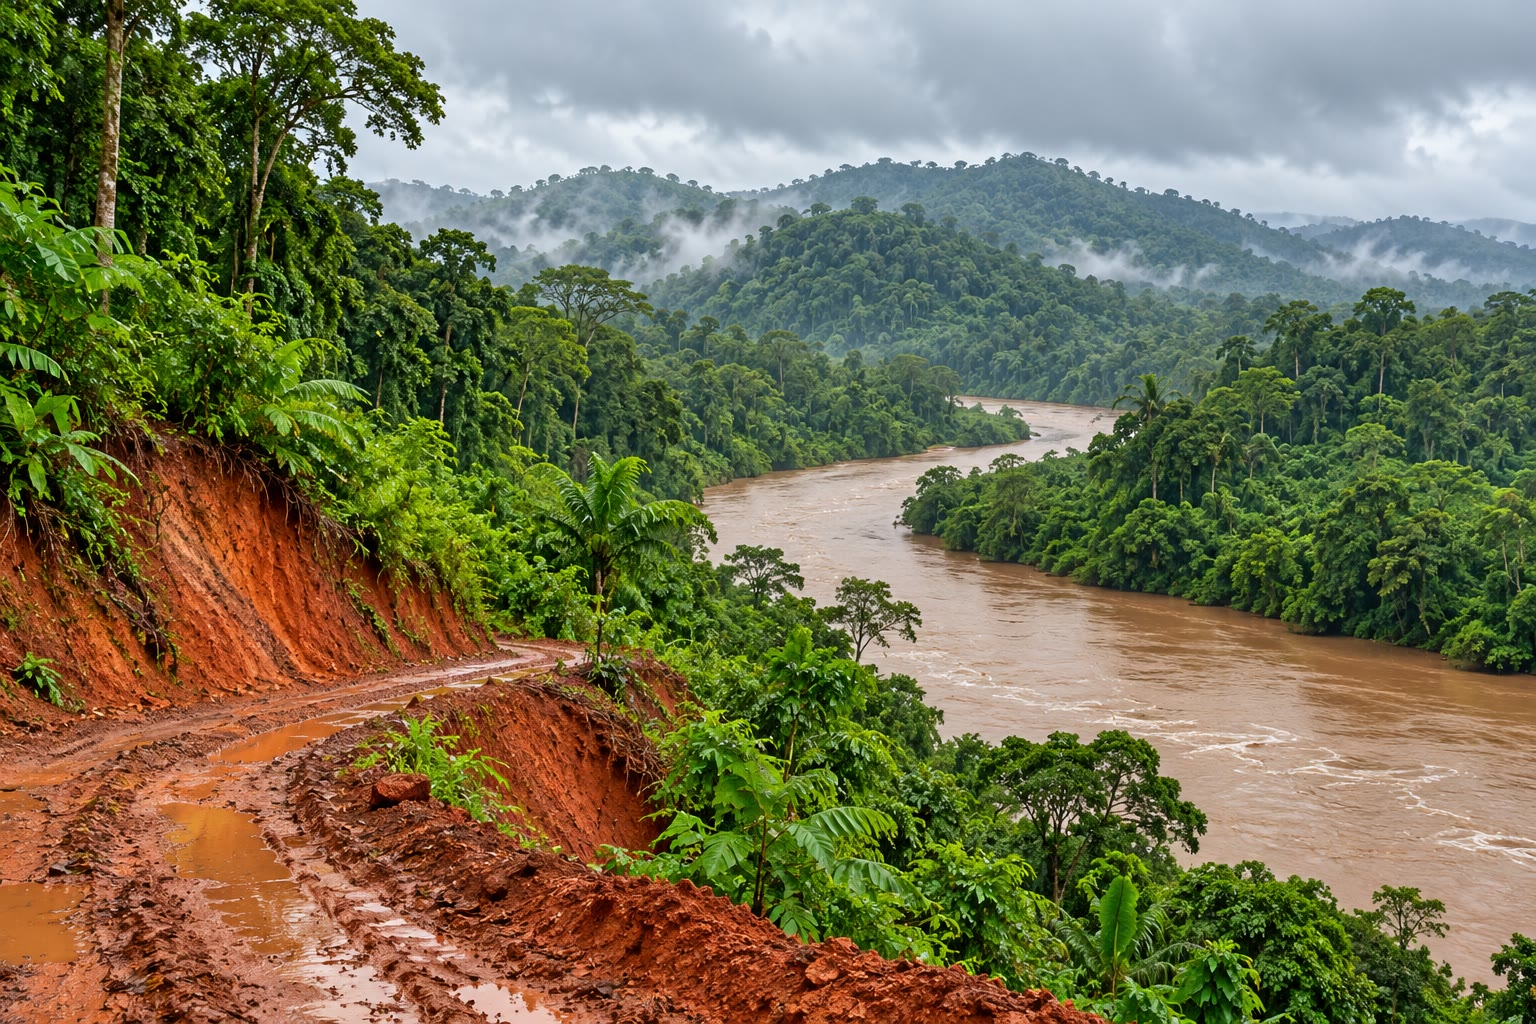
\includegraphics[width=0.66\linewidth]{images/book4/ai/b2-tropical-weathering.jpg}
\par\smallskip{\small Tempat termostat bekerja paling keras: dataran rendah yang panas dan basah, tempat hujan jatuh di atas
tanah merah yang lapuk dalam dan sungai membawa produk pelapukan ke laut
(ilustrasi buatan AI).}
\end{omfigure}

\section*{Latihan}\label{sec:b2:deep-time-climate:exercises}

Data untuk latihan, kecuali dinyatakan lain: karbon praindustri di atmosfer
\qty{591}{PgC} (\qty{278}{ppm}); $\qty{1}{Tmol}$ karbon $= \qty{0.012011}{PgC}$; pelapukan
silikat $W_0 = \qty{0.138}{PgC.yr^{-1}}$; bagian kelebihan yang tetap di udara setelah samudra dan
karbonat $f = 0.08$; kepekaan pelapukan $k_T = \qty{0.09}{K^{-1}}$; sensitivitas iklim $S =
\qty{3}{K}$; gaya radiatif penggandaan karbon dioksida \qty{3.93}{W.m^{-2}}; $R =
\qty{8.314}{J.mol^{-1}.K^{-1}}$.
% ledger: ar6ch5:fig512, ipcc:erf-2xco2, derry24:fluxes, colbourn13:timescale, colbourn13:weathering, ipcc:ecs

\begin{exercise}[$\star$]\label{exo:b2:deep-time-climate:1}
Sebelum era industri samudra memuat \qty{900}{PgC} di lapisan permukaannya, \num{37100} di air
menengah dan air dalamnya, 700 sebagai karbon organik terlarut, dan 3 dalam organisme hidupnya.
(a) Berapa banyak karbon yang dimuat samudra, dan berapa kali karbon atmosfer? (b) Konversikan
\qty{3.5e6}{Tmol} di reservoir permukaan ke petagram karbon. (c) Berapa bagiannya yang berada di
udara?
\end{exercise}

\begin{exercise}[$\star$]\label{exo:b2:deep-time-climate:2}
Gunakan fluks pada gambar \omterm{def:b2:deep-time-climate:carbon-cycle}{siklus karbon jangka panjang}, dengan pelepasan gas metamorfik diambil sebesar
\qty{3}{Tmol.yr^{-1}}. (a) Jumlahkan masukan ke reservoir permukaan dan keluarannya.
(b) Berapa bagian masukan yang dipasok oleh gunung api, celah, dan \omterm{def:b2:metamorphic-facies:metamorphism}{metamorfisme}? (c) Tentukan waktu
tinggal karbon di reservoir permukaan, dengan memakai keluarannya.
\end{exercise}

\begin{exercise}[$\star$]\label{exo:b2:deep-time-climate:3}
(a) Tuliskan pelapukan forsterit, \ce{Mg2SiO4}, oleh karbon dioksida dan air menjadi ion magnesium
dan ion bikarbonat serta silika terlarut, \ce{SiO2}, lalu setarakan. (b) Magnesium itu kemudian
diendapkan sebagai karbonat. Tuliskan reaksi bersihnya. (c) Berapa massa forsterit yang harus lapuk untuk
memindahkan \qty{1}{PgC} untuk selamanya? ($M(\ce{Mg2SiO4}) = \qty{140.7}{g.mol^{-1}}$.)
\end{exercise}

\begin{exercise}[$\star$]\label{exo:b2:deep-time-climate:4}
Urutkan menurut umur, beserta tanggalnya, dan nyatakan untuk masing-masing apakah Bumi berada dalam keadaan rumah kaca atau
rumah es: Optimum Iklim Eosen Awal; glasiasi Hirnantium; awal lembaran es
Antarktika; Turonium; luas es terbesar pada Paleozoikum akhir; kemajuan besar
lembaran es utara; PETM.
\end{exercise}

\begin{exercise}[$\star\star$]\label{exo:b2:deep-time-climate:5}
(a) Periksalah bahwa energi aktivasi \qty{63}{kJ.mol^{-1}} pada \qty{288}{K} memberikan $k_T =
\qty{0.09}{K^{-1}}$. (b) Tentukan $k_T$ untuk nilai lapangan \qty{74}{kJ.mol^{-1}}. (c) Dengan masing-masing, tentukan
pemanasan tunak ketika pelepasan gas naik \qty{20}{\percent}. (d) Mengapa sensitivitas
iklim tidak muncul dalam (c)?
\end{exercise}

\begin{exercise}[$\star\star$]\label{exo:b2:deep-time-climate:6}
Bandingkan faktor Arrhenius eksak $\exp[-(E_{\text a}/R)(1/T - 1/T_0)]$ dengan $e^{k_T(T -
T_0)}$, $k_T = E_{\text a}/(RT_0^2)$, untuk $E_{\text a} = \qty{63}{kJ.mol^{-1}}$ dan $T_0 =
\qty{288}{K}$: (a) pada $T = \qty{293}{K}$; (b) pada $T = \qty{318}{K}$. (c) Tunjukkan bahwa perbandingan
pendekatan terhadap faktor eksak adalah $\exp[E_{\text a}x^2/(RT_0^2(T_0 + x))]$, dengan $x = T - T_0$,
dan tentukan pemanasan saat perbandingan itu mencapai 1.1.
\end{exercise}

\begin{exercise}[$\star\star$]\label{exo:b2:deep-time-climate:7}
Kompilasi yang dihaluskan memberikan \qty{1444}{ppm} karbon dioksida pada \qty{419.5}{Ma} dan
\qty{276}{ppm} pada akhir rekamannya. (a) Tentukan gaya radiatif penurunan itu. (b) Bandingkan dengan
\qty{9}{W.m^{-2}} dari Matahari yang makin terang. (c) Tentukan laju penurunan rata-rata dalam ppm per juta
tahun, dan bandingkan dengan \qty{3.4}{ppm} dari tren hasil pencocokan. Mengapa keduanya dapat berbeda?
\end{exercise}
% ledger: data:b4-foster2017, foster17:co2

\begin{exercise}[$\star\star$]\label{exo:b2:deep-time-climate:8}
(a) Sebarkan \num{3000} dan \qty{7000}{PgC} selama 3 dan selama \qty{20}{ka}: rentang laju pelepasan
berapa yang dihasilkan? Bandingkan dengan 0.3 sampai \qty{1.5}{PgC.yr^{-1}} yang dikutip IPCC. (b) Emisi manusia
adalah sekitar \qty{35}{Gt} karbon dioksida pada 2010. Konversikan ke karbon dan bandingkan. (c) Karbon
dioksida naik dari 900 ke \qty{2000}{ppm}. Tentukan gaya radiatif dan pemanasan kesetimbangannya dengan $S =
\qty{3}{K}$, dan bandingkan dengan pemanasan \qty{5}{\celsius} di atas iklim pra-PETM.
\end{exercise}
% ledger: ar6ch5:petm-release, usgs:volcanic-co2, ar6ch5:petm

\begin{exercise}[$\star\star$]\label{exo:b2:deep-time-climate:9}
Naiknya suatu sabuk pegunungan mengalikan kemampuan lapuk Bumi $W_0$ dengan 1.2, pada pelepasan
gas yang tetap. (a) Tentukan perubahan suhu tunak yang baru. (b) Tentukan karbon dioksida tunak yang baru, dari
\qty{278}{ppm}. (c) Apakah laju pelapukan silikat, pada keadaan tunak yang baru, berbeda dari
laju yang lama? Jelaskan.
\end{exercise}

\begin{exercise}[$\star\star\star$]\label{exo:b2:deep-time-climate:10}
(a) Tentukan waktu e-folding termostat dengan faktor limpasan, $k = 0.09 + 0.65\times0.045$.
(b) Selama jutaan tahun lembaran es dan vegetasi juga menanggapi; dengan sensitivitas sistem
Bumi sebesar \qty{8}{K} per penggandaan sebagai pengganti $S$, tentukan $\tau$ dengan $k_T$. (c) Ke arah mana kedua
perubahan itu mendorong termostat, dan ketidakpastian mana, $E_{\text a}$ atau $S$, yang lebih penting?
\end{exercise}

\begin{exercise}[$\star\star\star$]\label{exo:b2:deep-time-climate:11}
Pelepasan \qty{5000}{PgC} (setelah samudra dan karbonat). (a) Tentukan karbon dioksida
udara, dalam ppm, dan pemanasannya. (b) Tentukan laju pemindahan bersih awal $W - W_0$, dan waktu yang diperlukan
pulsa itu untuk lenyap dengan laju tersebut. (c) Tentukan waktu yang dilinearkan untuk memindahkan \qty{90}{\percent}
kelebihan itu. (d) Model itu, bila diintegrasikan tanpa dilinearkan, memerlukan \qty{340}{ka}. Mengapa lebih lama?
\end{exercise}

\begin{exercise}[$\star\star\star$]\label{exo:b2:deep-time-climate:12}
(a) Linearkan model itu di sekitar keadaan tunak dengan pelepasan gas $V$ dan $C = C^*$, lalu tunjukkan bahwa
waktu e-folding-nya $\tau' = A_0 (C^*/C_0)\ln 2/(f k S V)$. (b) Hitunglah untuk keadaan tunak
akibat kenaikan pelepasan gas sebesar \qty{20}{\percent}. (c) Apakah termostat lebih cepat atau lebih lambat di dunia yang kaya
karbon dioksida, dan mengapa?
\end{exercise}

\begin{problem}[{Soal akhir pekan --- Berapa lama termostat bekerja?}]\label{pb:b2:deep-time-climate:1}
Soal ini membangun konstanta waktu termostat dari fluks-fluks yang terukur. Gunakan data
latihan; pelepasan gas di punggung samudra, \omterm{def:b2:oceanic-islands:stages}{pulau samudra}, busur, dan celah \num{1.3}, \num{1.3}, 4.5, dan
\qty{4.2}{Tmol.yr^{-1}}; pelapukan silikat 11 sampai \qty{12}{Tmol.yr^{-1}}; energi aktivasi
\qty{63}{kJ.mol^{-1}} pada $T_0 = \qty{288}{K}$; massa atmosfer \qty{5.1e18}{kg}, massa molar
rata-rata udara \qty{28.97}{g.mol^{-1}}. Bulatkan sampai tiga angka penting.

\noindent\textbf{Bagian I --- Keseimbangan.}
\begin{enumerate}
  \item Jumlahkan pelepasan gas gunung api dan celah, dalam \unit{Tmol.yr^{-1}} dan dalam \unit{PgC.yr^{-1}}.
  \item Ambil $W_0$ di tengah rentangnya; konversikan ke \unit{PgC.yr^{-1}}.
  \item Bandingkan keduanya. Apa yang disarankan perbandingan itu tentang \omterm{def:b2:deep-time-climate:carbon-cycle}{siklus karbon jangka panjang}?
  \item Berapa mol udara yang dimuat atmosfer? Berapa mol karbon dalam \qty{591}{PgC},
        dan berapa rasio campurannya?
  \item Tanpa pelapukan sama sekali, berapa lama pelepasan gas pada pertanyaan 1 akan menambahkan
        \qty{591}{PgC} ke reservoir permukaan?
  \item Jika fraksi $f = 0.08$ dari karbon itu tetap berada di udara, dengan faktor berapa karbon dioksida udara
        akan naik?
\end{enumerate}

\noindent\textbf{Bagian II --- Melinearkan.}
\begin{enumerate}[resume]
  \item Tentukan $k_T$ dari energi aktivasi, dan periksalah bahwa nilainya dibulatkan menjadi
        \qty{0.09}{K^{-1}} yang dipakai di bawah.
  \item Dengan faktor berapa pelapukan bertambah untuk pemanasan sebesar \qty{1}{K}?
  \item Tuliskan pemanasan $\Delta T$ untuk kelebihan $M$, dan turunannya pada $M = 0$, dalam
        \unit{K.PgC^{-1}}.
  \item Tentukan turunan $W$ terhadap $M$ pada $M = 0$, dalam \unit{yr^{-1}}.
  \item Tunjukkan bahwa kebalikannya adalah konstanta waktu $\tau$ pada
        \cref{prop:b2:deep-time-climate:thermostat}.
  \item Mana di antara $f$, $k$, $S$, dan $W_0$ yang membuat termostat lebih cepat bila nilainya bertambah?
\end{enumerate}

\noindent\textbf{Bagian III --- Konstanta waktu.}
\begin{enumerate}[resume]
  \item Hitunglah $\tau$.
  \item Hitunglah dengan faktor limpasan, $k = \qty{0.119}{K^{-1}}$.
  \item Hitunglah dengan $k_T$ dan energi aktivasi \qty{74}{kJ.mol^{-1}}.
  \item Bandingkan nilai-nilai ini dengan \qty{200}{ka} sampai \qty{1}{Ma} dari model dengan samudra yang eksplisit.
  \item Berapa banyak waktu e-folding yang muat dalam \qty{50}{Ma} penurunan karbon
        dioksida Kenozoikum? Apa artinya bagi keadaan siklus karbon selama penurunan itu?
  \item Pada \qty{16}{ppm} per juta tahun, berapa besar perubahan karbon dioksida dalam satu $\tau$?
\end{enumerate}

\noindent\textbf{Bagian IV --- Pelepasan seukuran PETM.}
\begin{enumerate}[resume]
  \item \qty{5000}{PgC} dilepaskan; berapa banyak yang tetap berada di udara setelah samudra dan karbonat
        bertindak, dan berapa karbon dioksidanya dalam ppm?
  \item Tentukan pemanasan pada saat itu.
  \item Seberapa besar laju pelapukan naik, dalam \unit{PgC.yr^{-1}} dan dalam persen?
  \item Dengan hukum yang dilinearkan, berapa lama sampai \qty{90}{\percent} kelebihan itu hilang?
  \item Karbonat PETM pulih selama sekitar \qty{100}{ka}. Berikan dua alasan mengapa Bumi yang sebenarnya
        mungkin lebih cepat daripada model ini.
  \item Sebagai ringkasan: berapa waktu e-folding \omterm{def:b2:deep-time-climate:thermostat}{termostat pelapukan silikat} dalam model ini?
\end{enumerate}
\end{problem}
% ledger: derry24:fluxes, colbourn13:weathering, colbourn13:timescale, ar6ch5:fig512, ar6ch5:petm, ar6ch5:cenozoic-co2, ipcc:ecs, earth:Matm, earth:Mmol
